%%%%%%%%%%%%%%%%%%%%%%%%%%%%%%%%%%%%%%%%%%%%%%%%%%%%%%%%%%%%%%%%%%%%%%%%%%%%%%%%
%2345678901234567890123456789012345678901234567890123456789012345678901234567890
%        1         2         3         4         5         6         7         8

\documentclass[letterpaper, 10 pt, conference]{ieeeconf}  % Comment this line out if you need a4paper

%\documentclass[a4paper, 10pt, conference]{ieeeconf}      % Use this line for a4 paper
                                   % Needed to meet printer requirements.

% See the \addtolength command later in the file to balance the column lengths
% on the last page of the document

% The following packages can be found on http:\\www.ctan.org
\usepackage{graphics} % for pdf, bitmapped graphics files
\usepackage{epsfig} % for postscript graphics files
\usepackage{multirow} 
\usepackage{subcaption}
\usepackage{caption}
\usepackage{url}
\usepackage{bnf}
\usepackage{slashbox}
\newcommand{\co}{\cellcolor{gray!40}}
\usepackage[table]{xcolor}
%\usepackage{mathptmx} % assumes new font selection scheme installed
%\usepackage{times} % assumes new font selection scheme installed
%\usepackage{amsmath} % assumes amsmath package installed
%\usepackage{amssymb}  % assumes amsmath package installed
\IEEEoverridecommandlockouts                              % This command is only needed if 
                                                          % you want to use the \thanks command

\overrideIEEEmargins   

\title{\LARGE \bf
Enriching Robot's Actions with Affective Movements
}


\author{Julian M. Angel-Fernandez$^{1}$ and Andrea Bonarini$^{2}$% <-this % stops a space
\thanks{$^{1}$Julian M. Angel-Fernandez is a Research at Automation and Control Institute, Vienna University of Technology, Vienna, Austria
        {\tt\small julian.angel.fernandez@tuwien.ac.at}}%
\thanks{$^{2}$Andrea Bonarini is a Professor at the Department of Electronics, Information, and Bioengineering, Politecnico di Milano, Milan, Italy,
        {\tt\small andrea.bonarini@polimi.it}}%
}


\begin{document}



\maketitle
\thispagestyle{empty}
\pagestyle{empty}


%%%%%%%%%%%%%%%%%%%%%%%%%%%%%%%%%%%%%%%%%%%%%%%%%%%%%%%%%%%%%%%%%%%%%%%%%%%%%%%%
\begin{abstract}
Emotions are considered by many researches as a characteristic that could be beneficial in social robotics, since they enrich human-robot interaction with non-verbal clues. Although there have been works that have studied emotion expression in robots, mechanism to generate emotion are highly integrated with the rest of the system. This unable the possibility to use their approaches in different applications. This paper present a system that has been initially created for a theatrical robot to enrich with emotions its actions, but it has been designed to enable the possibility to be adapted to be used in other fields. The emotional enrichment system has been envisioned to be used with a action decision system. A formal description of the system is provided to be used as a formal reference for further extensions and possible modifications. The system has been adapted to two different platforms with different grades of freedom: Keepon and Triskarino. 
\end{abstract}

\section{Introduction}
The development of fast, cheap, and reliable electronics has enabled the creation of new devices and versatile robotic platforms. These new platforms' capabilities have expanded the frontiers of the robots applications  to new environments where robot are expected to interact with humans, such as health care, and house cleaning, among others. However, bringing robots in these environment raises the challenge to increase robots' acceptance. Although this could be seen as an easy task that just would need improvements in robots' appearances and capabilities, it is possible that people would expect to treat robots as humans has  as they do with computers.~\cite{Reeves1996}, which makes necessary the creation of robots that fulfil this expectations.

Some researchers have suggested that embedding emotion expression capabilities to robots could improve their acceptance in social environments~\cite{Pavia2014}. As consequence researchers~\cite{Breazeal2002,Arras2012} have added specific emotional poses and expression to their robots. Others have studied how to convey emotions with specific platforms~\cite{Li2011,Brown2014}. Nevertheless, these works have created modules to show emotions that are strongly integrated to their solutions, which eliminate the possibility to re-use or adapt their systems into other projects.

In theory, the projection of emotion with humanoid embodiments could be simplified to mimic the same movements that humans. However, this idea is not possible due robots physical limitations. Therefore, an exact matching of humans’ movements to convey emotions could not be used in robots \cite{Saerbeck2007,Canamero2010}. Therefore diverse researchers are studying diverse features and values to express emotions with different platforms. As a consequence, these results could not be widely used due to the differences of the platforms.

This paper presents an Emotional Enrichment System (EES), which modify actions' parameters and add additional actions to create the illusion of emotion expression in a robot. Although the EES was originally conceived to be used in an autonomous performance robot~\cite{angel2013} to enrich actions with emotions, its design was devised to make it extendable to other platforms and adaptable to new tasks. To achieve this goal, the system relies on an Emotional Execution Tree (EXT), which is based on simple actions, sequential and parallel nodes. Additionally, it is used the concept of compound actions to group a bunch of nodes, which reduces the tree dimension and allows the reuse of recurrent actions  generated by specific combinations of simple actions and other nodes. This EXT has been formalized to give a guideline to further implementations and extensions.
 
The rest of the paper is organized as follows. Section~\ref{sec:related_work} provides a brief overview of particularly relevant work related to our system. Section~\ref{ref:theatre} gives a brief explanation on TheatreBot architecture. Section~\ref{ref:general_system} gives a general introduction to the system ideas. Section~\ref{sec:emotional_execution_tree} gives the basic formalization of our system and principal components terms used on it. Section~\ref{sec:implementation} describes the implementation of the system and shows two demonstrations done with the system using platforms with different capabilities.
\section{Related Work}
Most of the works done in Human-Robot Interaction (HRI) have focused on faces, due to the abundance of works in face elicitation in humans. One of the most well-known expressive robots is Kismet~\cite{Breazeal2002}, a robotic face able to interact with people and to show emotions. The face had enough degrees of freedom to portray the basic emotions suggested by Ekman~\cite{Ekman2004} (\textit{Happiness}, \textit{Surprise}, \textit{Anger}, \textit{Disgust}, \textit{Fear}, and \textit{Sadness}), plus interest. 
Despite the complex system behind Kismet, the emotion's projection evaluation was done using videos with a very limited number of participants. Similar approach was followed by Li and Chignell~\cite{Li2011}, who used videos of a teddy bear robot to study the contribution of arms and head movement to express emotions. In same direction Destephe and collaborators~\cite{Destephe2013} studied the attribution of emotion to a robot's gait using a virtual representation of the platform WABIAN-2R. Knight and Simmons~\cite{knight2016} used two platforms (i.e. Keepon and NAO) with different degrees of freedom to study the possibility to project inner states with just head movements. Although the use of videos has the advantage to cover a major number of participants, they loss the impact that is created from the interaction between the participant and the platform.

%%%%%%%%%%%%%%%%%%%%%%%%
The use of real platforms to study emotion projection could be dissect by the type of platform used. Therefore two tendencies could been observed: use of anthropomorphic and non-anthropomorphic platforms. In the first case, these works are characterized by the use of cue positions to project desire emotions~\cite{NAO2013}. In some cases, special attention has been taken to determine head's angle and arms position contribution in specific emotions~\cite{Brown2014}. 
Nevertheless, current humanoid platforms cannot generate smooth gaits, which limit the study of body movements. To overcome this limitation, some researchers have reduce the human appearance (e.g. eliminating limps and facial expressions)to increase platform mobility and study new mechanisms to project emotions~\cite{Arras2012}. Trying to reduce the anthropomorphism, Saerbeck and Christoph used a Roomba platform to study the contribution of curvature in a trajectory to conceive emotional states~\cite{Saerbeck2010}. Similarly Lourens and Barakova~\cite{BarakovaL10} implemented a set of behaviors to determine the emotion  perceived from diverse movements, which were selected from the  work done by Camurri et al.~\cite{pop00002}. Continuing with her research on how robotics' behaviours are interpreted by people, Barakova and collaborators~\cite{Barakova2013} created a closet in which lights could be manipulated to convey pre-defined behaviours. The robot's behaviours were defined using the Interpersonal Behaviour Circle (ICB)~\cite{Leary57}, which is based on two dimensions (dominance-submission and hate-love). Their findings suggest that electronic systems can elicit a type of reactions different from the one expected by theories of interpersonal communication.

Other approaches have tried to get a better understanding of the contribution of diverse features to express emotions through movement. For example, Suk and collaborators payed a particular attention to speed, smoothness, granularity of movement path and volume of a non-bioinspired object~\cite{NAM2014}. Their results suggest that arousal increases as speed increases and that there is not any clear tendency for smoothness. On the other hand, granularity is positively correlated with pleasure and arousal, while volume is negatively correlated with pleasure and positively correlated with arousal. Alike, Tan and collaborators~\cite{Tan2016} have studied the contribution of velocity, fluidity, direction and orientation of a small box. Their results suggest that direction is directly correlated with dominance, but that fluidity does not influence the perception. While flat orientation is related to positive valence, leaning position are related with negative valance. Finally the velocity is correlated with valence, arousal and dominance.  

Due to the popularity that quadrocoptors have received in the last years, Sharma and collaborators~\cite{Sharma2013} used a quadrotor to study how different Laban's effort~\cite{Laban1968} parameters could impact on the perception of affection. A professional Laban certified actor was asked to generate 16 different paths, for each one changing one of the four Laban's parameters (space, weight, time, and flow). Each generated path was recorded using the Vicon motion-tracking system. Continuing with the use of quadrocoptors, Cauchard and collaborators~\cite{Cauchard2016} studied how flight paths could project personal traits and emotional attributes. All these works present a very nice starting to point to identify features and values that could be used to project emotions in robotics, which could help in coordinating humans and robots~\cite{Novika2015}. However, these works not give a price guideline to elicit precise emotions. This could lead to implementations that express a not desired emotion~\cite{Angel2016}. For example people could confuse an implementation of \textit{Happiness} with \textit{Anger}.
\section{Basic Concepts}
\label{sec:concepts}
The system is based on six main concepts: \textit{simple actions}, \textit{compound actions}, \textit{action message}, \textit{emotional descriptors}, \textit{character description} and \textit{emotional execution tree}. \textit{Action message} establishes the structure of the message to describe any kind of action (i.e., simple and compound). This message also specifies how the actions are executed (i.e., in parallel or in sequence) and which action is predominant (i.e., primary or secondary). \textit{Emotional parameters} describe how the emotional enrichment should be done to convey a specific emotion in a specific simple action. This description could also include addition of other simple actions. \textit{Character description} enables the possibility to establish how to modify emotional expressions to generate diverse treats. Finally, \textit{Emotional Execution Tree} is a computational representation of desired actions that should be executed. This tree is first created from the action message description and then modified using the emotional parameters and character description.  
\subsection{Simple and Compound Actions}
In order to generate a system that could be used in diverse platforms require an abstraction level in which all of them could fall. Therefore simple and compound actions are used to achieve this goal. Simple actions are actions that are considered as primitives: they are used as building blocks. Therefore, these actions are described in the system and are the ones in which the emotional enrichment takes place. Their description specifies mandatory and optional parameters that are required to execute an action. Compound actions are actions that are created from simple actions. These actions are not implemented in the system, but, if it is needed, they can be described in it (e.g. compound actions that are used often).

The simple actions to be implemented to test the system were selected by considering platforms' capabilities and the requirements. The eight actions selected are: move body, oscillate body, move shoulder, oscillate shoulder, move torso, oscillate torso, and do nothing. Description for each action, its mandatory parameters and optional parameters are shown in Table~\ref{table:actions_implemented}.

\begin{table}
\centering
\caption{Description of the seven simple actions implemented, and their respective parameters. Where  P is 2D position, V is 2D velocity vector and angular velocity, and T is time}
\label{table:actions_implemented}
\begin{tabular}{|c|p{3.9cm}|p{1.4cm}|}
\hline
\textbf{Action Name}& \textbf{Description} &\textbf{Parameter(s)} \\
\hline
Do nothing & It waits for a time $t$ before it is terminated. It could be seen as a delay.  & $T$\\
\hline
Move body & It moves the platform from its current position $a$ to a desired position $b$. & $P$, and $V$\\
\hline
Oscillate body & It generates an oscillation in the whole platform by an angle $\theta$. &  $\theta$ and $V$ \\
\hline
Move shoulder & It moves the shoulders to a desired angle $\theta$. It is considered as angular movement. & $\theta$ and $V$ \\
\hline
Oscillate shoulder & It oscillates the shoulders by a given angle $\theta$ & $\theta$ and $V$\\
\hline
Move torso & It moves the torso to a desired angle in $yaw$, $pitch$ and $roll$& $yaw$, $pithc$, $roll$ and $V$\\
\hline
Oscillate torso & It oscillates the shoulders by a given angle $\theta$ & $\theta$ and $V$\\  
\hline
\end{tabular}
\end{table}

%TODO add an example for this, very simple and presenting how to do it 
\section{Describing Components}
The description files allow the parametrization of the system and its adaptation to different circumstances. The system has the following parametric data:

\begin{itemize}
%TODO In the following the term "parameter" is misleading. A parameter should be a number, which doees not seem to be for all teh features you are describing. all teh descriptions are really unclear.
	\item \textit{Emotion description} gives the values of the parameters that should be changed in all the simple actions to express the desired emotion. Therefore, for each emotion-action combination, a description of how the parameters are defined and how they change in time should be provided. 
%If there is any action that does not have any specification, the system will not change its parameters. 
Four descriptors to describe any emotional movement are provided. %TODO I cannot understand this first descriptor
The first is the reference, which informs the system about the velocity used to calculate the parameter. This reference is used to let the modulation of the parameters depending on the character. The second descriptor is the tuple space and time. used to compute the velocity of the movement required to convey the desired emotion. %TODO I canot understand the following sentences. All this paragraph is confused and grammatically incorrect
in order to enable the possibility to have different velocities during the execution, it could be described a sequence of this tuple. In this case, the space descriptor plays the important role of stating the amount of space for which the desired velocity must be used. This brings the last description which is the repetition that is used if there is more than one tuple and it should be repeat during the duration of the movement. The EBFN to describethese descriptors in the system is the following: 
\begin{grammar}
[(colon){$\models$}]
[(semicolon)$|$]
[(comma){}]
[(period){\\}]
[(quote){\begin{bf}}{\end{bf}}]
[(nonterminal){$\langle$}{$\rangle$}]
<emotion description>: "'\{'","'emotion:'",<string> "','","'observation:'",<string> "','",<action>"'(,'",<action>)* "'\}'".
<action>:<string>"':\{'",<description> "','",<actions affected> "'\}'".
<description>:"'description:\{'",<action name>"','",<emotion>"','"\\
<parameter's type>"'\}'".
<action name>:"'emotionProfileAction:'",<string>.
<emotion>:"'emotionProfileEmotion:'",<string>.
<parameter's type>: "'movement\_parameter'".
<actions affected>:"'actions:\{'",<action parameter>,\\("','"<action parameter>)*"'\}'".
<action parameter>: <string>"':\{'",<reference>"','"\\<repetition>"','",<parameters>"'\}'".
<reference>: "'reference:'",<number>.
<repetition>: "'repetition:'","'yes'";"'no'".
<parameters>: "'parameters:['" <parameter description>\\("','",<parameter description>)* "']'".
<parameter description>: <movement parameter description>;<new parameters>.
<movement parameter description>:"'\{time:'",<number>"',space:'"\\<number>"'\}'".
\end{grammar}

	\item \textit{Character's emotions} parameters give the system information about character's ''rhythm'' for each pair action-emotion. To describe these changes, it was decided to use bias, amplitude and length as descriptors. Bias refers to a constant value that is added to the sequence of emotional parameters. Amplitude amplifies the velocity with respect to the bias if the number is bigger than one, or attenuate if it is between zero and one. 
%TODO if there is enough space add an image explaining these concepts


	\item \textit{Action message} contains all the necessary information for to execute an action. The following is the EBNF of an action:
\begin{grammar}
[(colon){$\models$}]
[(semicolon)$|$]
[(comma){}]
[(period){\\}]
[(quote){\begin{bf}}{\end{bf}}]
[(nonterminal){$\langle$}{$\rangle$}]
<action>: <simple action>;<compound action>;<context>.
<simple action>: "'\{'" <action header> "','","'parameters:['" <simple action parameters> "']\}'".
<compound action>: "'\{'" <action header> "','","'parameters:['" <compound action parameters> "']\}'".
<action header>: "'type:'", <action type> "','","'name: '" <string>  "','", <is primary>.
<simple action parameters>: "'\{'"<parameter header> "','" ,<parameter description> "'\}'". 
<compound action parameters>:  <simple action parameters> ("','", <simple action parameters>)* .
<context>:"'\{'" <action type> "','", <emotion sync> "','", <action sync> "','", <is primary> "','"\\" 'information:'", <string> "','"," 'actions: '", <action> "'\}'".
<parameter header>: "'type:'", <parameter type> "','"," 'name:'",<string>.
<parameter description>: <parameter amplitude>;<parameter circle>;<parameter landmark>;\\<parameter point>;<parameter speech>;\\<parameter square>;<parameter time>.
<parameter type>: "'mandatory\_parameter'";"'optional\_parameter'". 
<is primary>: "'yes'";"'no'".
<emotion sync>: "'yes'";"'no'".
<action type>: "'parallel\_context'";"'serial\_context'";"'simple\_action'";\\"'composite\_action'".
\end{grammar}
\end{itemize} 

\section{Emotional Tree}
Emotional Execution Tree is a connected acyclic graph $G(V,E)$ with $|V|$ vertexes and $|E|$ edges. The root and non-leaf nodes could be of either \textit{parallel} or \textit{sequential} type, which represent the type of actions that would be executed by the system. Sequential nodes execute one branch after the other. Once all the branches have been executed, asequential node notifies its predecessor to continue with the execution of other branches. The parallel node executes all the branches at the same time. This type of node offers two levels of synchronization: action and emotion. The action level synchronization enables the possibility to stop all the branches once the main branch has completed its execution. This main branch is established in the action message. On the other hand, the emotion level synchronization updates to a new emotional parameter of all the branches once the main branch updates to a new emotional parameter. %TODO The previous sentence is not clear. I cannot understando so I cannot fix it. What does it mean that updates to a parameter?
In both cases, any update or finish message will be ignored if the branch is not principal. These two levels of synchronization create four sub-types of parallel nodes: (i) action and emotion synchronous, (ii) action synchronous and emotion asynchronous, (iii) action asynchronous and emotion synchronous, or (iv) action and emotion asynchronous. 
 
Finally, leaf nodes are only simple action nodes that have been implemented in the system. Any node can belong to one of two levels: principal or secondary. If a node is principal, it will notify its predecessor about the messages that it has received, while the secondary node cannot propagate any message to its predecessor. This enables the possibility to have actions that have priority over others. To exemplify this, let us consider the sequence of actions depicted in Figure~\ref{fig:sequence_actions}. The Emotional Execution Tree for this sequence would be like the one presented in Figure~\ref{fig:emotional_enrichment}.

\begin{figure}
	\centering
	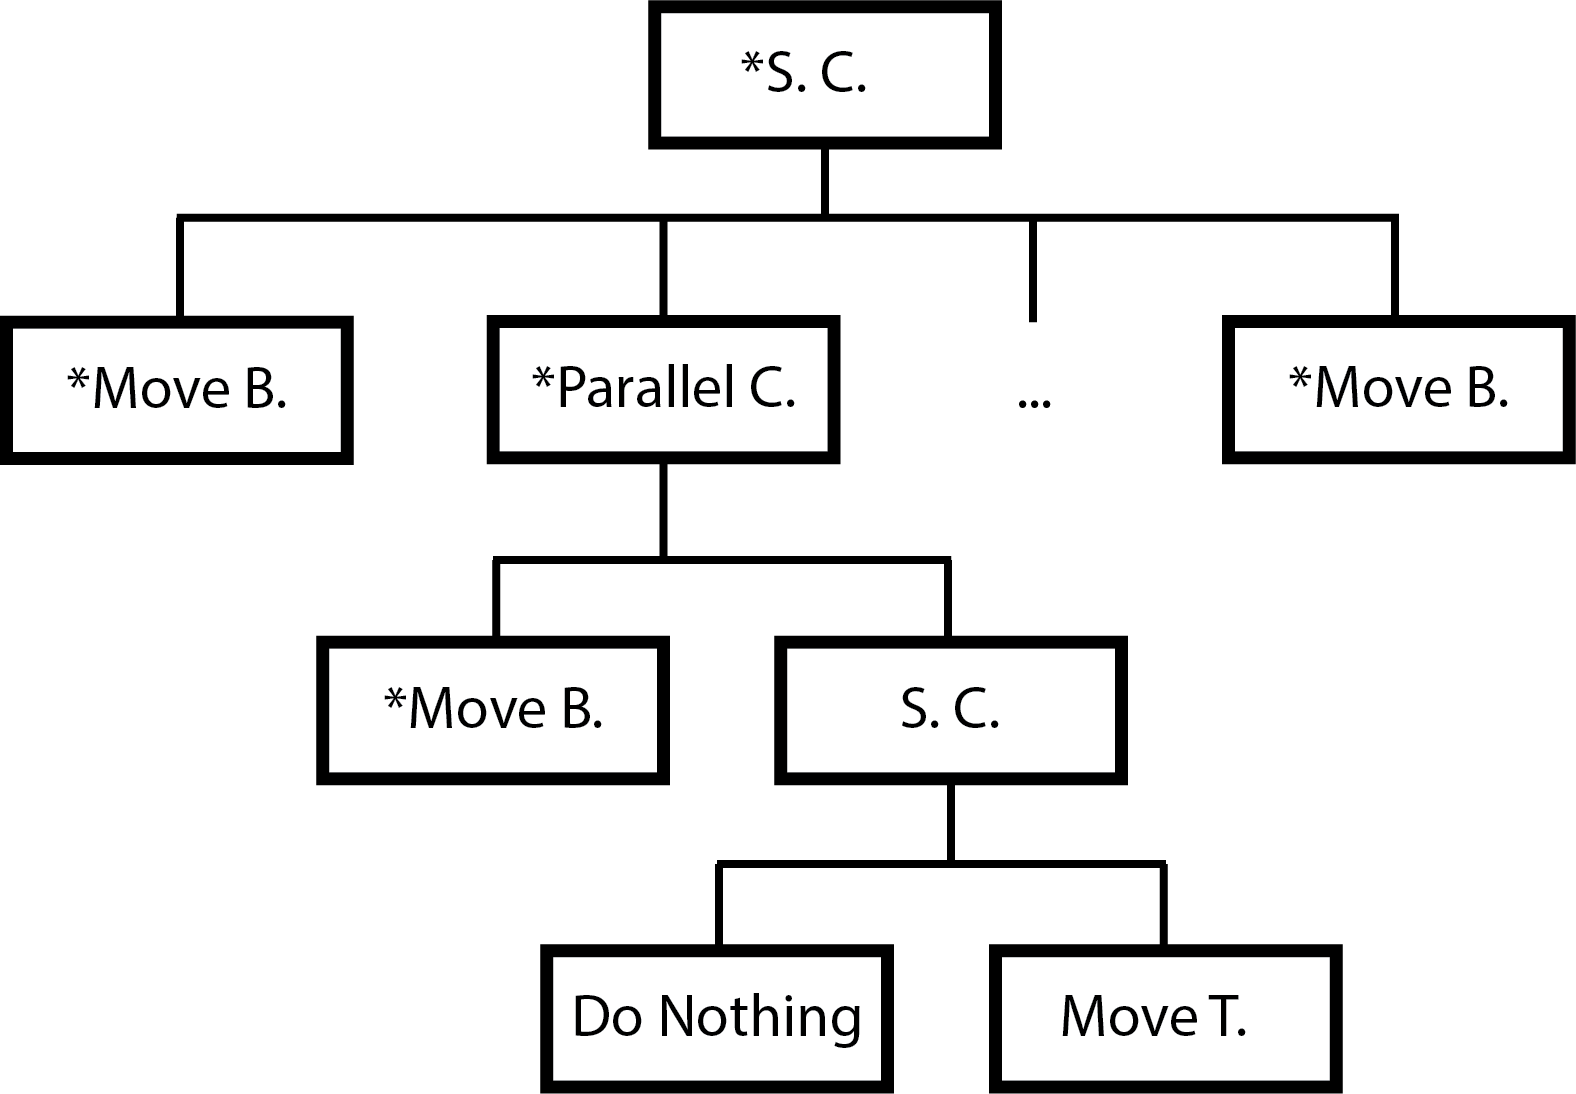
\includegraphics[width=0.45\textwidth]{./Images/Representation.png}
	\caption{Emotional Execution Tree for the sequence of actions depicted in Figure~\ref{fig:sequence_actions}. The $*$ symbol denotes principal nodes. $S$ represents sequential.}
	\label{fig:emotional_enrichment}
\end{figure}

\subsection{Formalization of Simple and Compound Actions}
Formalizing simple and compound actions enables the generation of a system to design them and verify if they are described correctly. Simple actions ($SA$) could be seen as functions that map a set of parameters $p^{pl}_{i} \in P$ to specific platform ($pl$) movements ($m^{pl}_{j}\in M^{pl}$) in the set of movements for that platform ($m^{pl}_{j} =sa^{pl}(\lbrace p^{pl}_{i} \rbrace)$). Each $sa^{pl}$ could have different implementations due to different reasons such as: platform's configuration, action's goal, how the mapping from inputs to outputs are done, among others. 
In our case, we consider that two actions are different if $(\forall sa_{i}, sa_{j} \in SA, \forall q, t \in PL | Param( sa_{i}^q ) \neq Param( sa_{j}^t )\Rightarrow sa_{i}^q \neq sa_{j}^t)$, 
where $PL$ is the set of all the possible platforms, $Param(\cdot)$ returns the set of parameters that are input of the $sa$ (e.g., $vel$,$pitch$,$text$). 
On the other hand, we will consider two actions as equivalents if $(\forall sa_{i}, sa_{j} \in SA , \forall q, t \in PL | Param( sa_{i}^q ) = Param(sa_{j}^t ) \wedge Obj(sa_{i}^q) = Obj(sa_{j}^t) \Rightarrow sa_{i}^q \equiv sa_{j}^t)$,  
where $Obj(\cdot)$ returns the set of objectives that are intended to be achieved by a given action. This $SA$ equivalence allows us to avoid the specification of all the platforms for all the actions that share the same objective and hide leaf nodes that do not give relevant information to understand the emotional tree.

With this $SA$ definition, it is now possible to define emotion enrichment as $ (\forall sa \in SA, \forall e \in E, \exists \; en$ $|$ $en=Enrichment(sa,e,Param(sa), Intensity(e)))$, where $Intensity(\cdot)$ returns the intensity of a given emotion, $E$ is the set of emotions, and $en$ can be the same $sa$, but with the parameters modified in order to convey the desired emotion $e$, or even a set of $sa$ with modified parameters. This definition goes along with the idea that new $sa$ could be added to convey a specific emotion. In addition, the $Enrichment(\cdot)$ function has the following properties:
\begin{itemize}
	\item $(\forall sa_{i},sa_{j} \in SA, \forall e \in E$ $|$ $sa_{i} \equiv sa_{j} \Rightarrow Enrichment(sa_{i},e,...) \equiv Enrichment(sa_{j},e,...))$
	\item $(\forall sa_{i},sa_{j} \in SA, \forall e \in E$ $|$ $(sa_{i} \not\equiv sa_{j}) \Rightarrow Enrichment(sa_{i},e,...) \not \equiv Enrichment(sa_{j},e,...))$
\end{itemize}

The concept of compound action ($CA$) is defined as $g = ca(\{p_{i}\})$, where $(p_{i} \in Param(sa))$, $(sa \subseteq SA)$, $(g \in EXT)$.

\section{Implementation}
The system was implemented in \textit{C++} and interfaced with ROS. The design (Fig.~\ref{fig:system_architecture}) was created following the description presented in the previous sections. 
\begin{figure*}
	\centering
	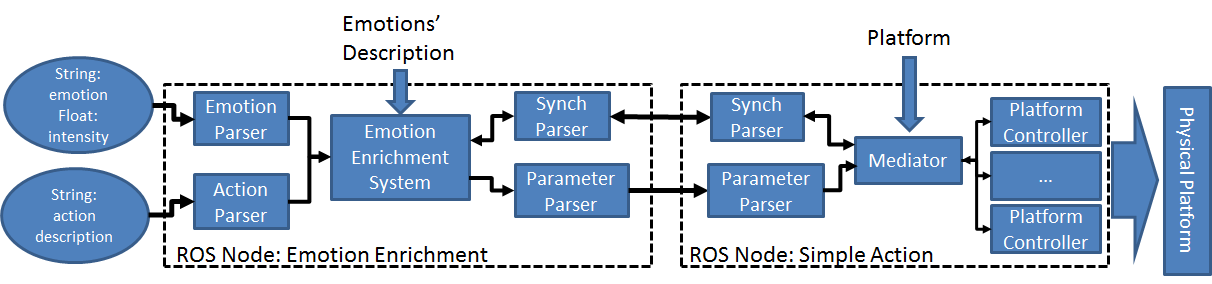
\includegraphics[width=1.0\textwidth]{Images/SystemArchitecture.png} 	
	\caption{General system design. Each simple action corresponds to one ROS node, and there is just one node for the emotion enrichment system. The ovals represent the ROS topic parameters, rectangles represent \textit{black boxes}, and texts outside containers represent input files that contain the system parametrization.}
	\label{fig:system_architecture}
\end{figure*}
The emotion enrichment core is divided in three different modules. 
Each module is responsible for one of the following phases:
\begin{enumerate}
	\item \textit{Generation of emotional execution tree:} this phase starts every time that a new action message is received. The process begins by parsing the format, verifying that the actions described on it exist in the system, and that the parameters correspond to the ones expected by each action included in the message. 
When the verification is done, and all the actions exist and the parameters correspond, an EXT such as the one presented in Figure~\ref{fig:emotional_enrichment} is created.
	\item \textit{Emotion addition:} uses the EXT created in the previous phase. In this phase new simple actions ($sa$)
can be added to the EXT, and the $sa$'s parameters are modified following the emotion description, which is loaded from files. This process is broken down in two steps. First, all the actions that are required to convey the desired emotion, and that are not yet present are added. Second, the emotional parameters are modulated basing on the emotion's intensity and character traits. The final EXT is presented in Figure~\ref{fig:reference}.
	\begin{figure}
		\centering
		%Representation
	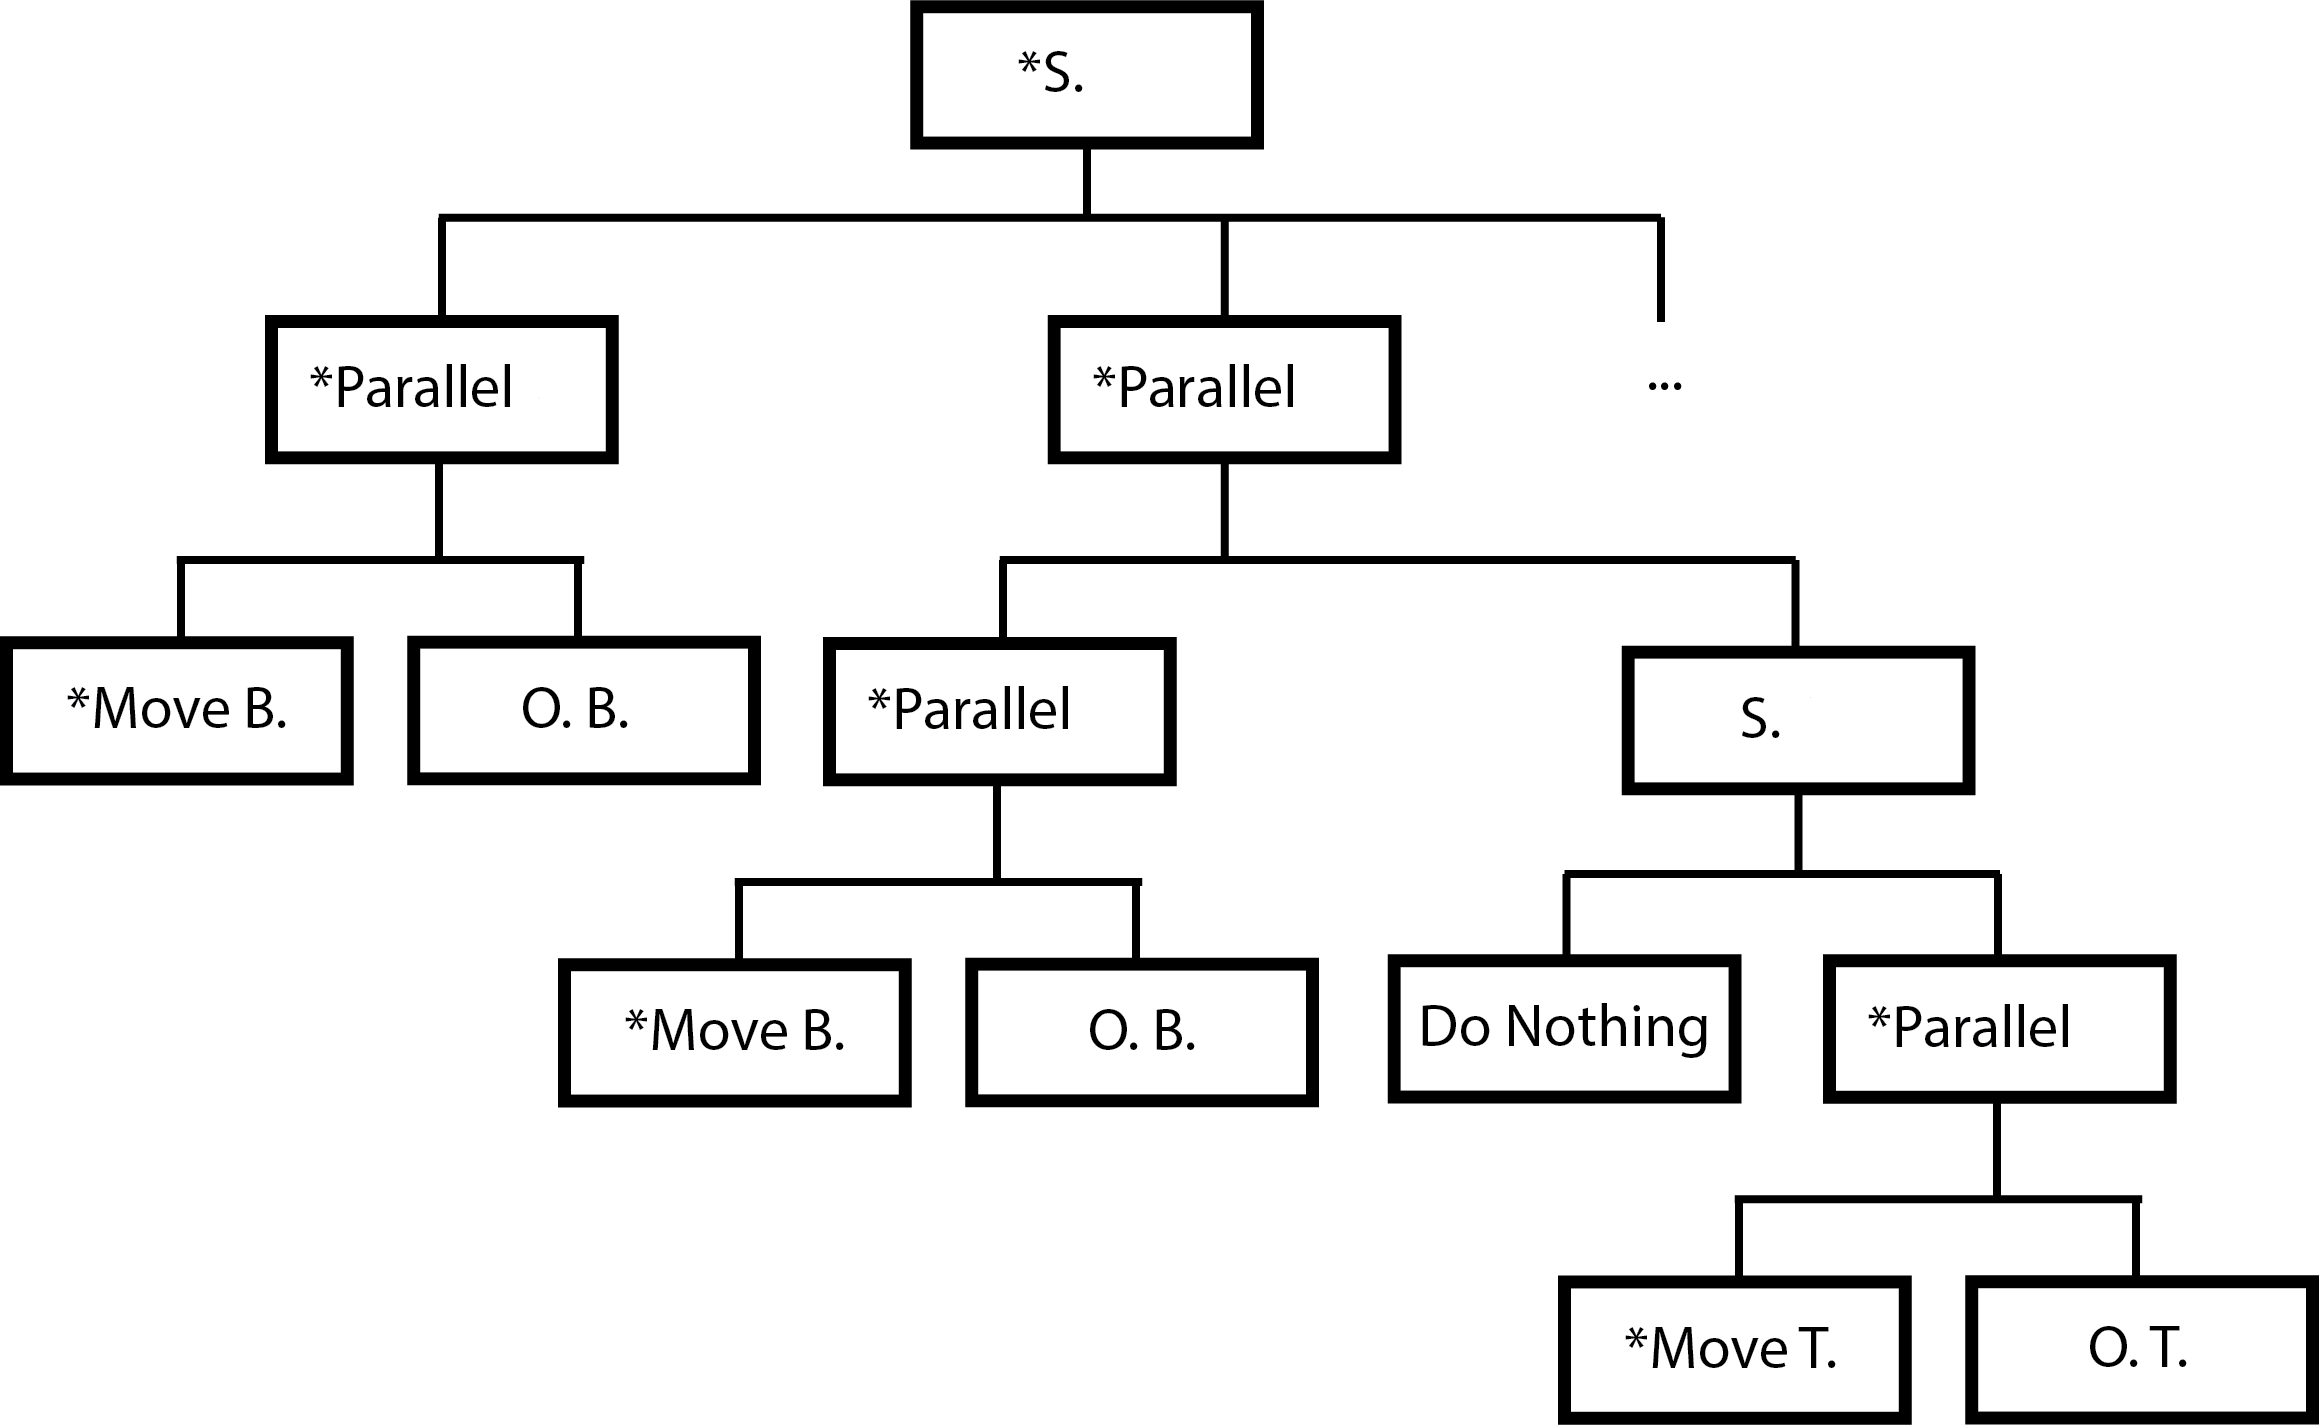
\includegraphics[width=0.45\textwidth]{./Images/exampleTreeE.png}
	\caption{EXT enriched with emotion for the EXT presented in Figure~\ref{fig:emotional_enrichment}.} 
	\label{fig:reference}
	\end{figure}
	\item \textit{Execution:} this is the last phase and it is done after the EXT is ''coloured'' with emotional features (actions additions and emotional parameters). The decision to have two different communication channels, one for action parameters and another for the action emotional parameters, was taken to enable the possibility to update the emotional parameters without interfering with the current execution. 
\end{enumerate}

All the text message broadcast among the nodes are written using JSON format, which is human understandable, light, and can be parsed by many systems.
 
To test the system, two different platforms were used: Keepon Pro~\cite{Kozima–2009}
and an own made platform called Triskarino.
Keepon has been used to test the interoperability of the system to different platforms, while Triskarino has been used in diverse case studies to explore emotion projection with a non anthropomorphic platform.
%%%%%%%%%%%%%%%%%%%%%%%%%
%%%%%%%%%%%%%%%%%%%%%%%%%%%%%
\subsection{Keepon Test}
To test the system with Keepon (Fig.~\ref{fig:keepon}), it was just necessary to implement the platform's controllers in each one of the simple action ROS nodes. Given that this platform does not have the capability to displace its body, the action ``move body'' was not implemented. Once added these controllers to the system, we proceeded to modify the configuration files to use this platform instead of Triskarino. With this small modification, we were able to change from one platform to other. In the video\footnote{YouTube video name Emotional Enrichment System, url: https://youtu.be/bRSXQ0rzkO8}
is shown the test where Keepon had to move its torso forward and backward to express a ``happy'' emotion. 
\begin{figure}
	\centering
	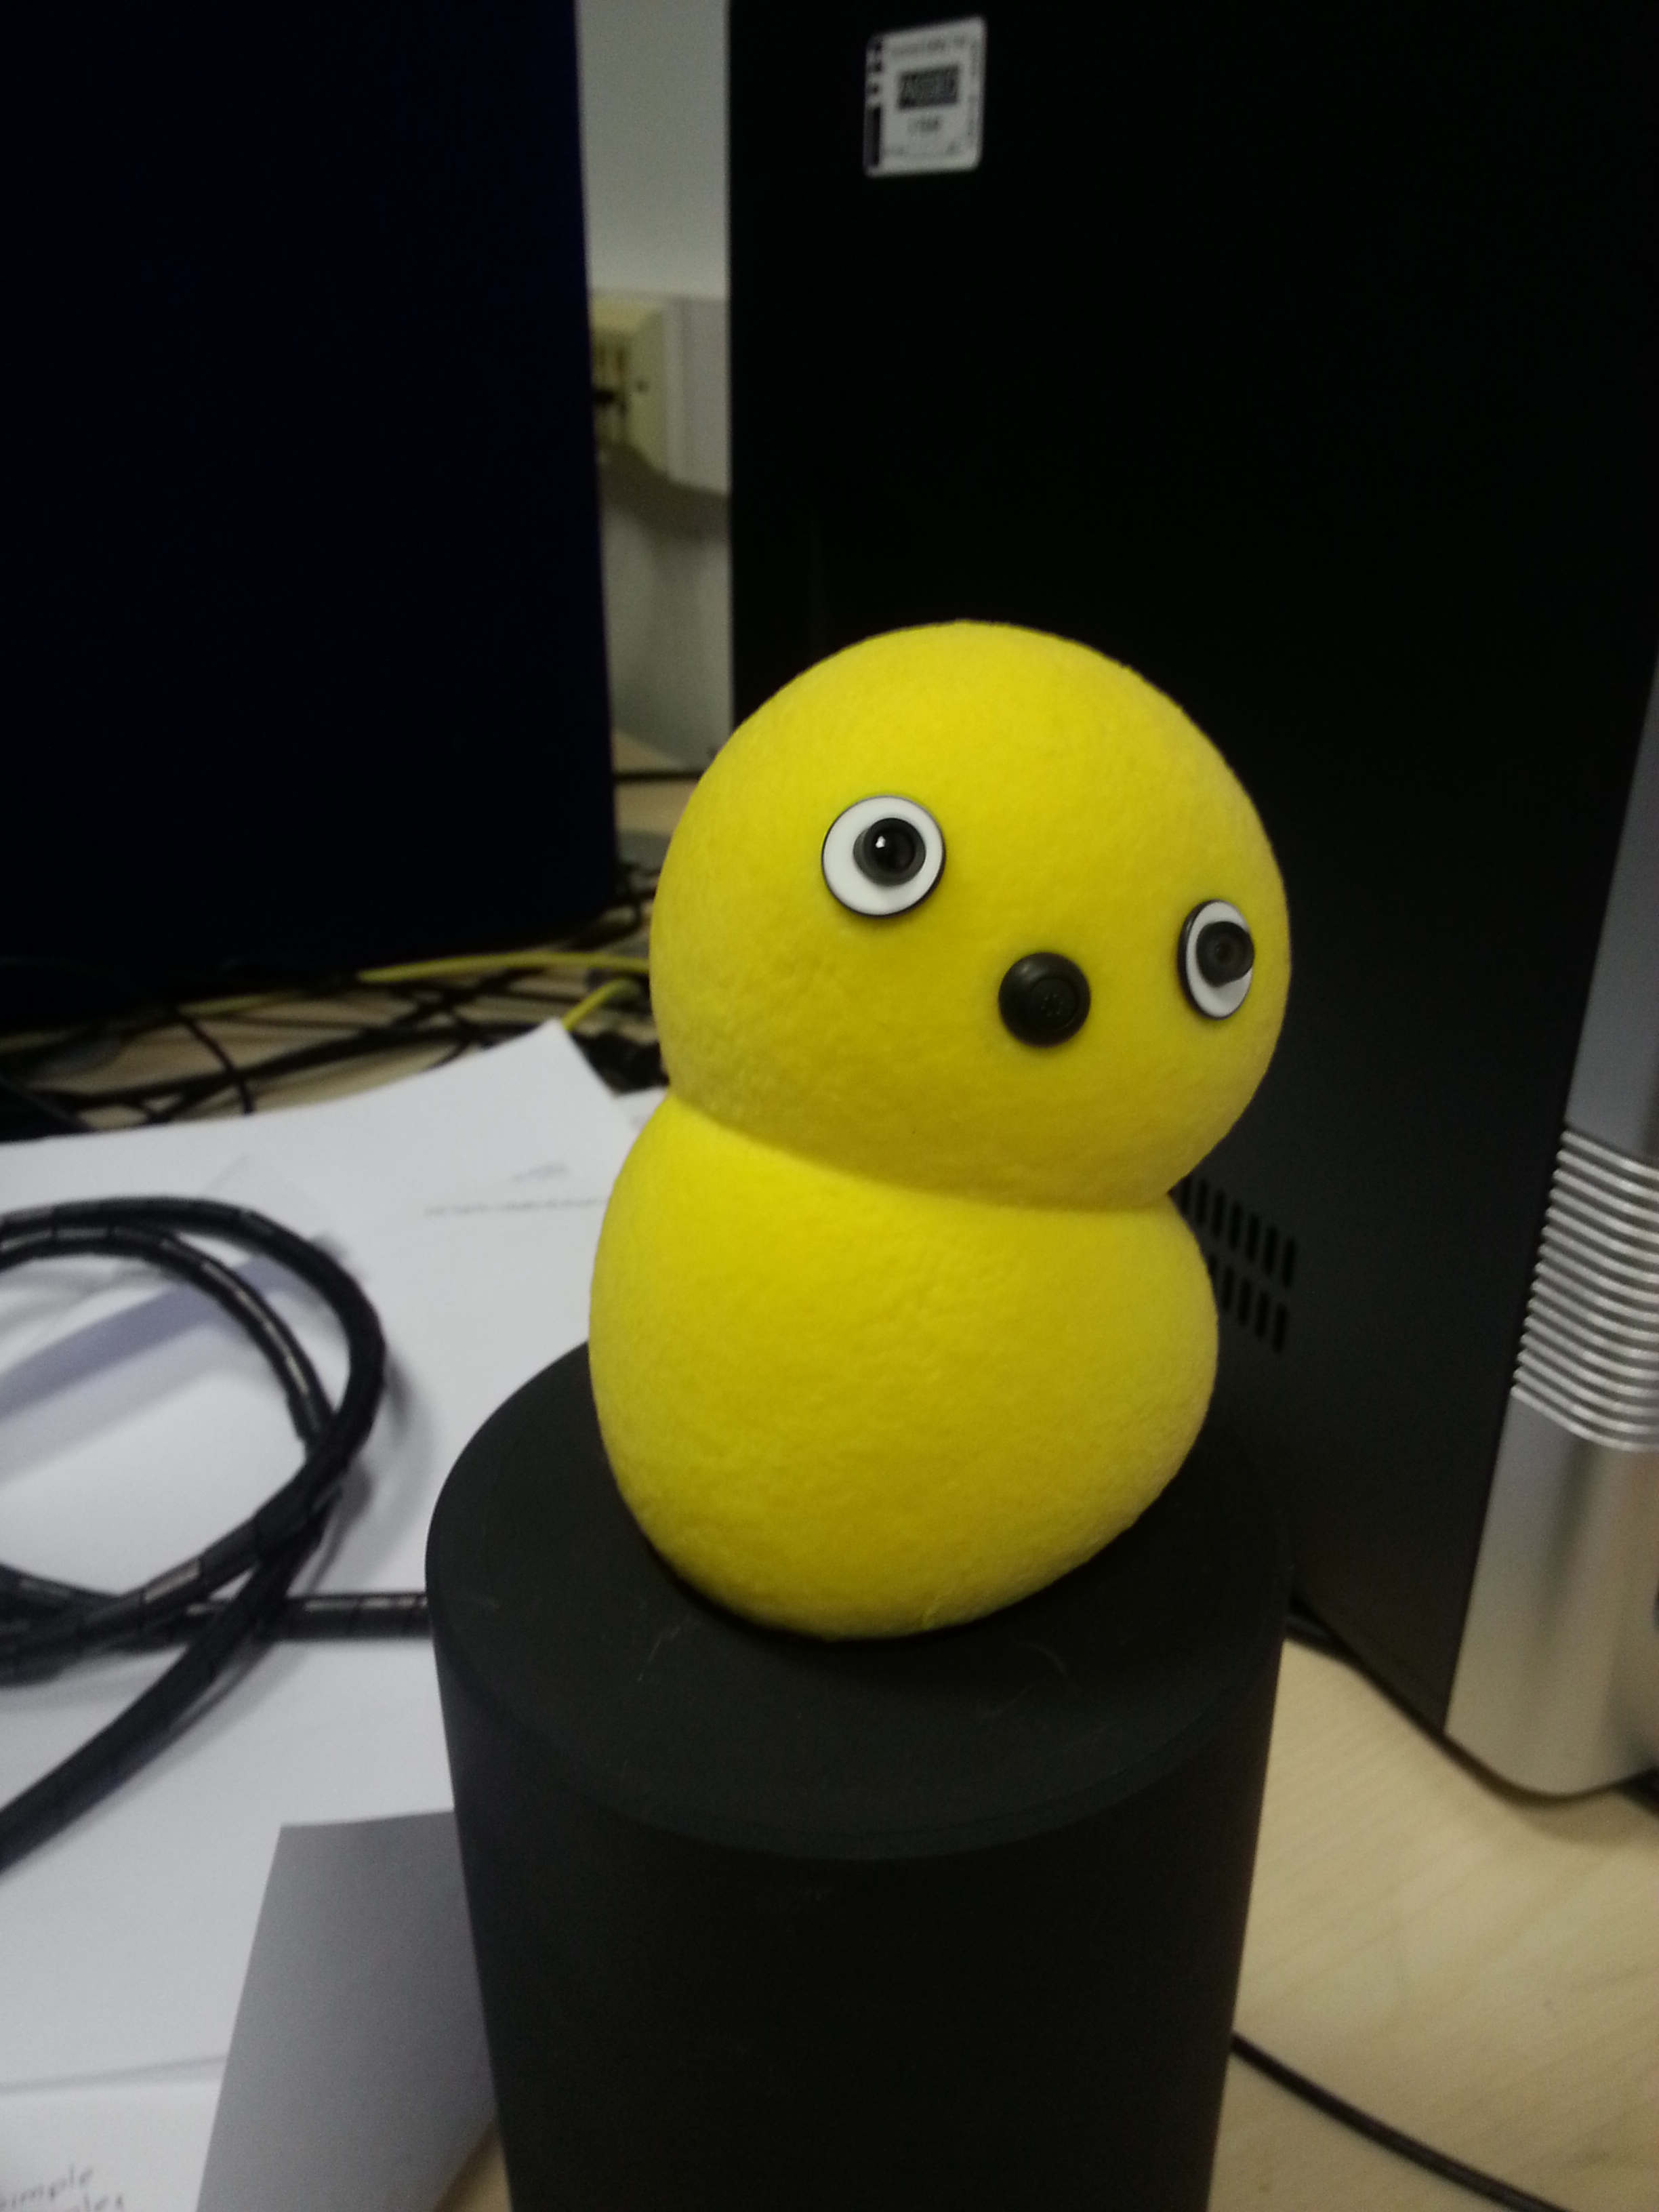
\includegraphics[width=0.2\textwidth]{./Images/Keepon.jpg}
	\caption{Keepon platform.}
	\label{fig:keepon}
\end{figure} 
The action is given by console telling the robot to bend the torso to a desired angle in x. The torso oscillation in y is added automatically by the system following the description defining how to express happiness. 
 %%%%%%%%%%%%%%%%%%%%%
%%%%%%%%%%%%%%%%%%%%%%%%%%%%%
\subsection{Triskarino Test}
The system has been widely used with Triskarino (Fig.~\ref{fig:robot}) during our studies on projecting emotions with a non human like platform~\cite{angel2017robots}. 
\begin{figure}
	\centering
	\begin{subfigure}[c]{0.2\textwidth}
	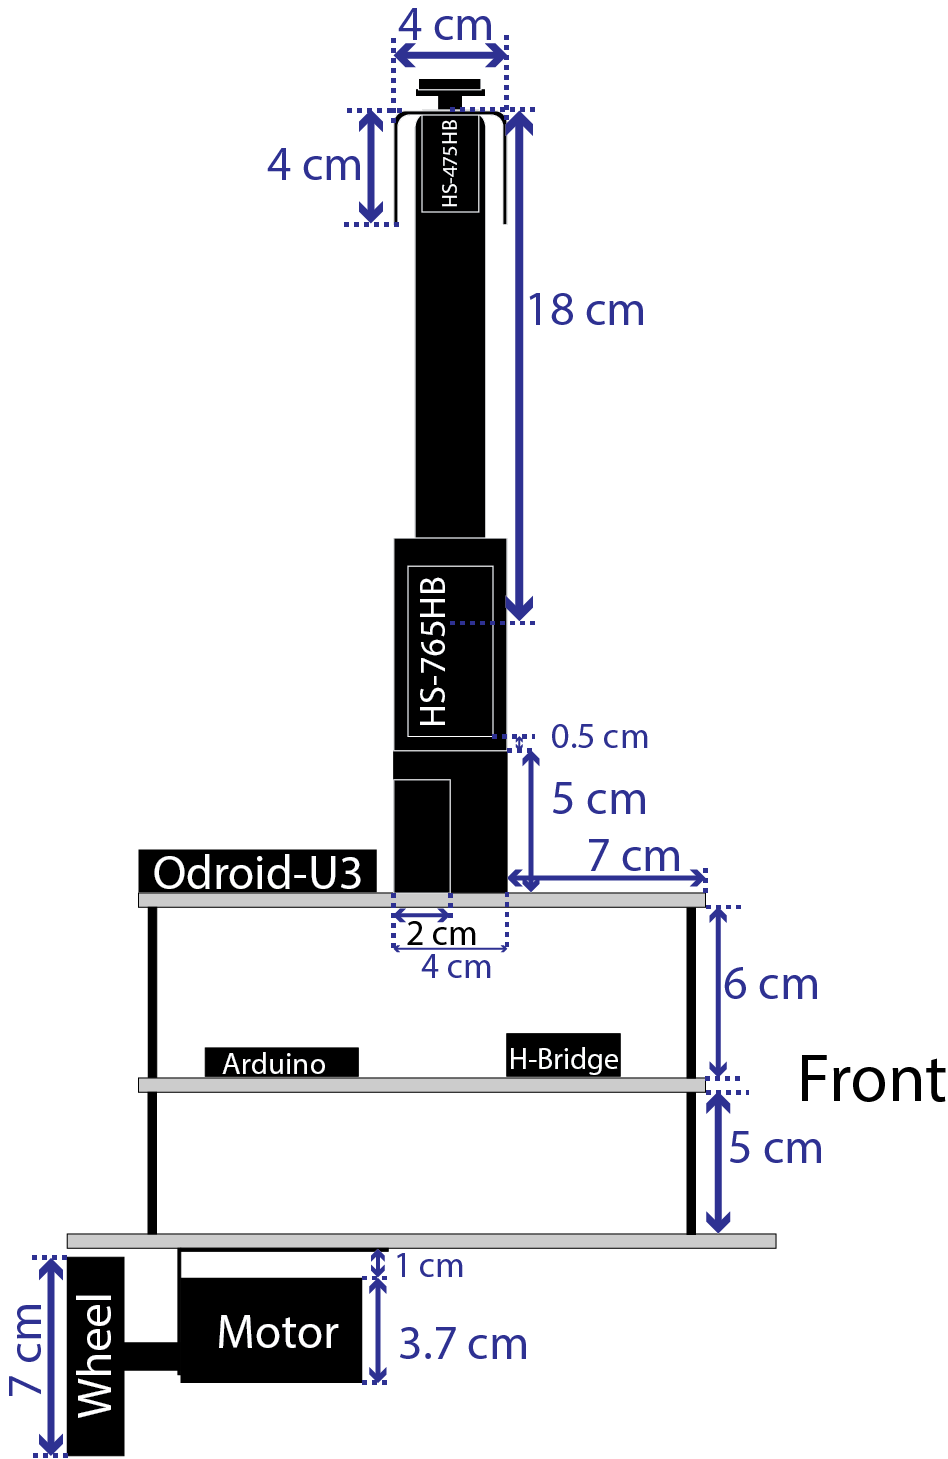
\includegraphics[width=\textwidth]{./Images/upperFourthD.png}
	\caption{Triskarino design.}
	\label{fig:design}
	\end{subfigure}
	\begin{subfigure}[c]{0.2\textwidth}
	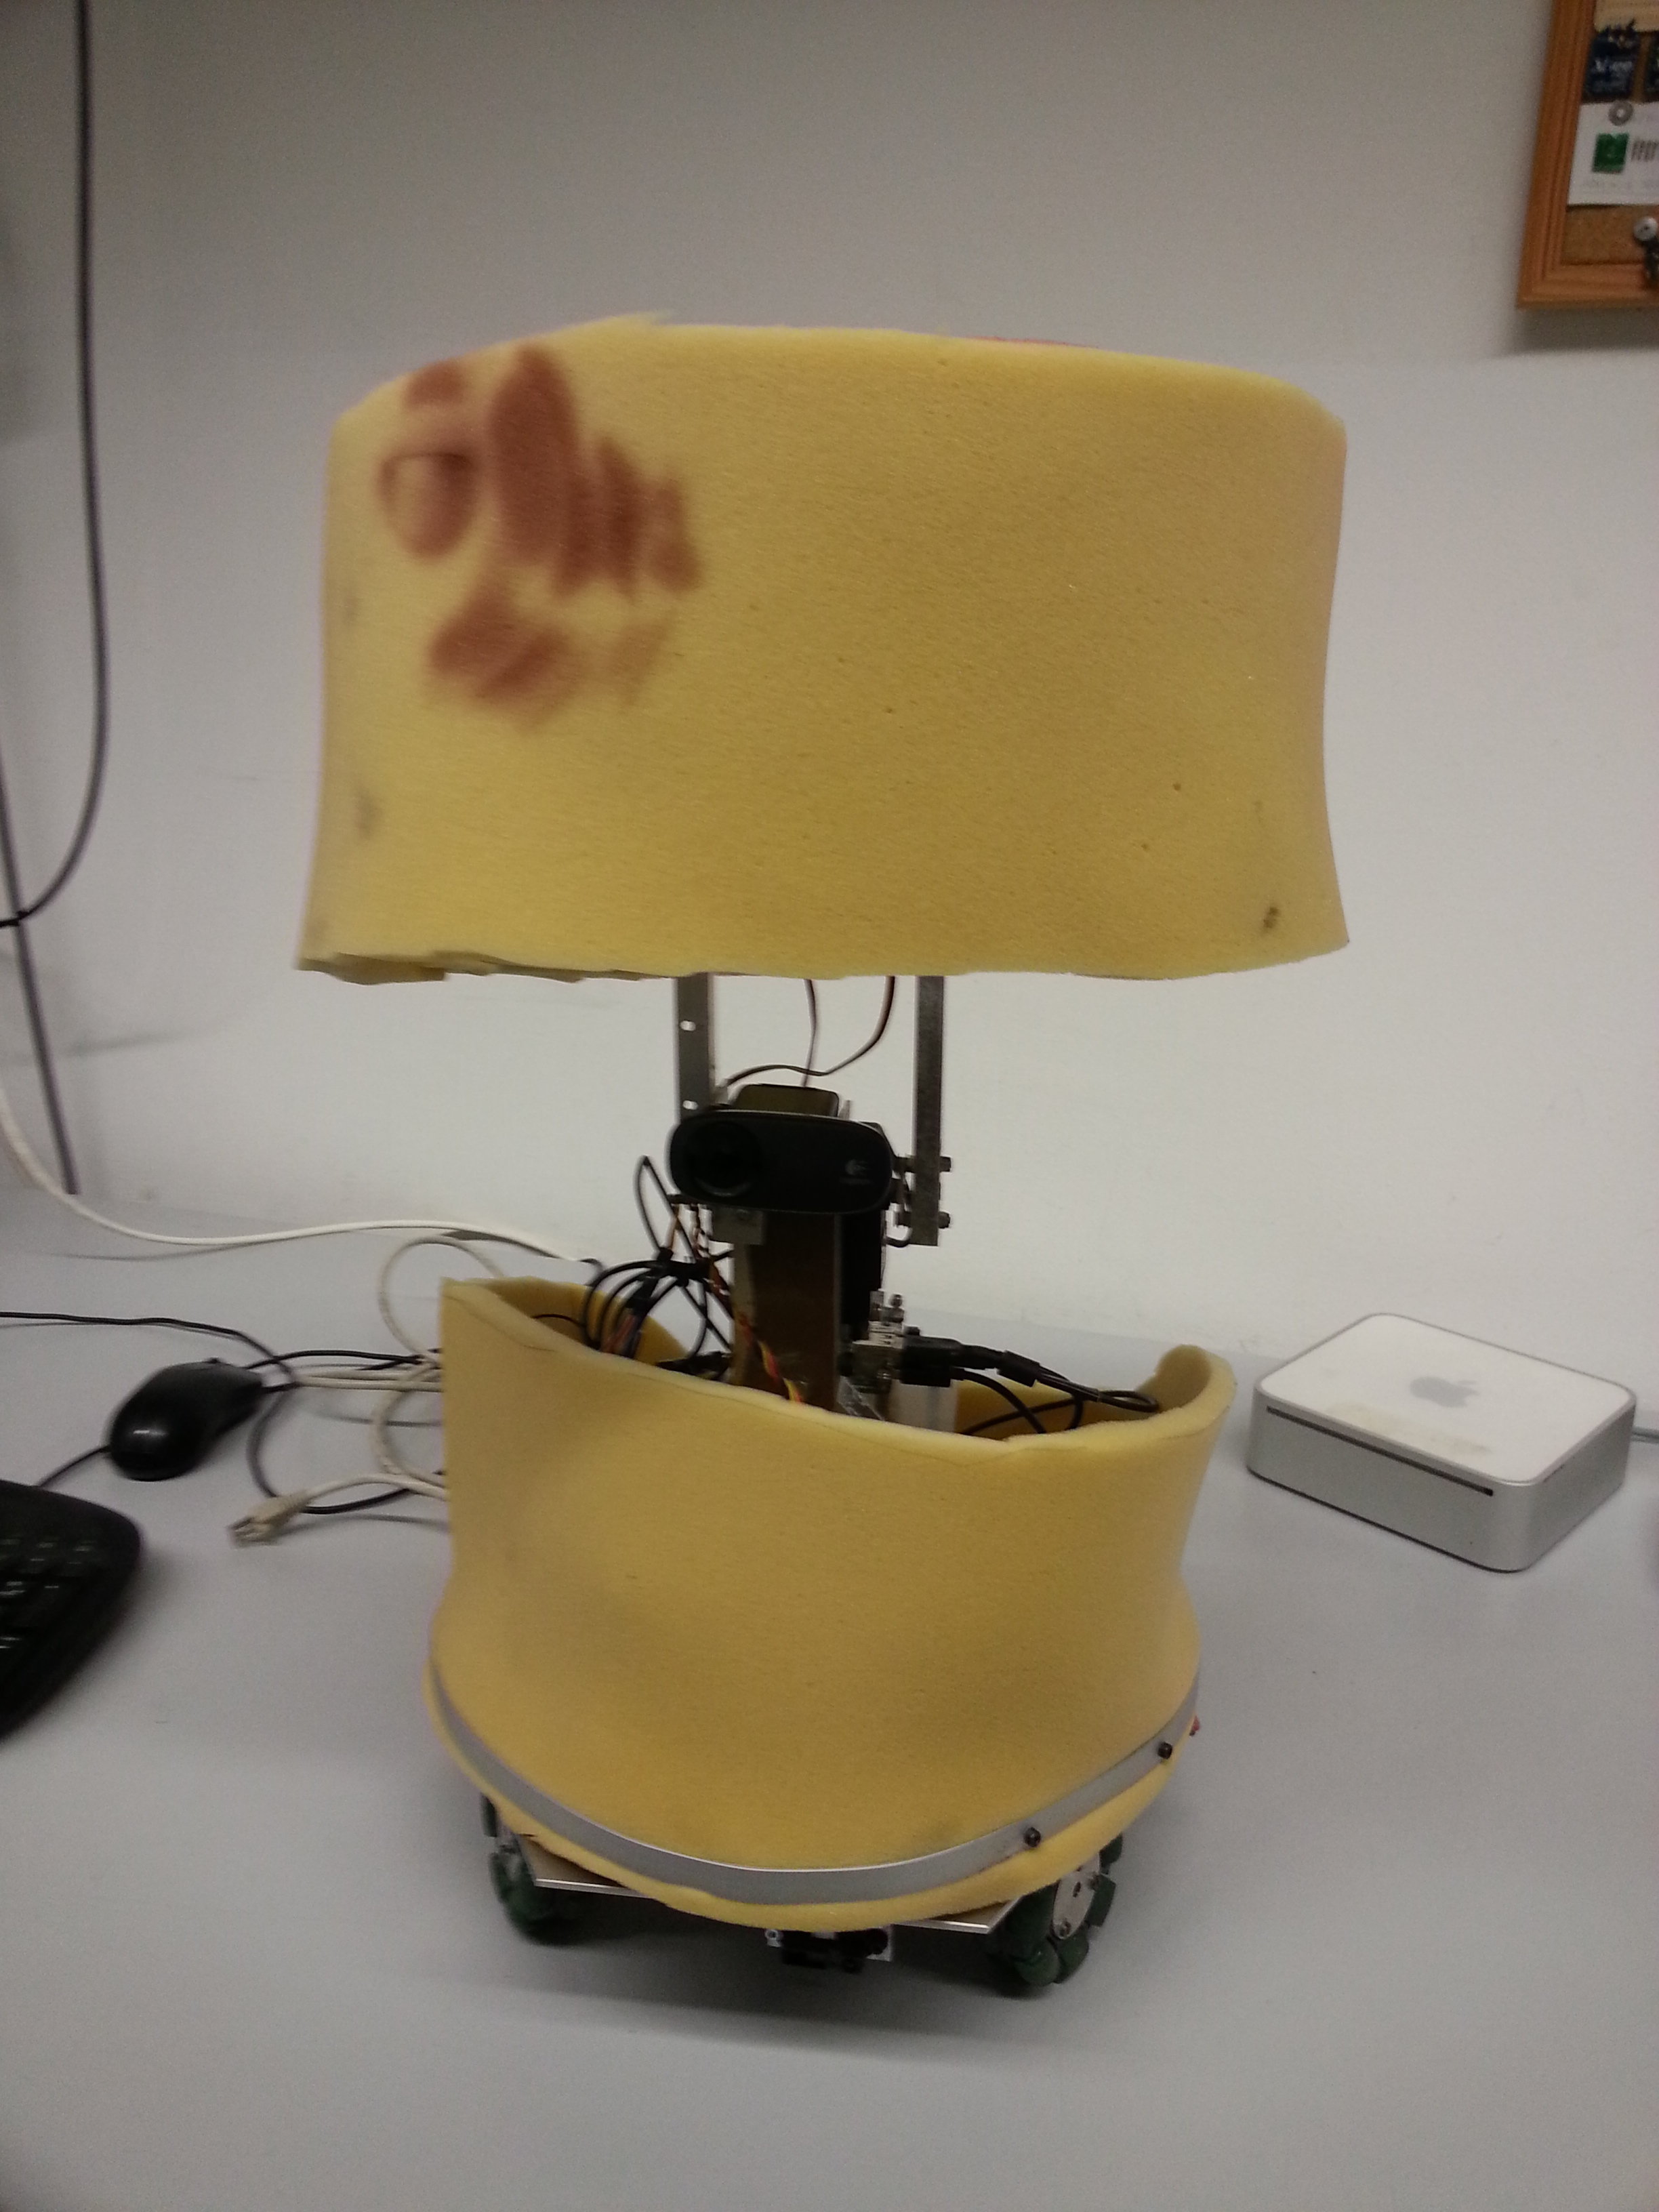
\includegraphics[width=\textwidth]{./Images/platform_fome.jpg}
	\caption{Triskarino with its cover.}
	\label{fig:triskar}
	\end{subfigure}
	\caption{Triskarino platform.}
	\label{fig:robot}
\end{figure}  
 In these studies, the system was used in different experiments to move the robot on a straight line showing different emotions, each one selected from our command console. Moreover, to show the whole capabilities of the emotional enrichment system and verify if it could be used in real time, a little scene was set up. The scene is a modification of the first part of the balcony scene of Shakespeare's Romeo and Juliet play~\cite{RAndJ}. The simplified sketch of our version could be seen in Figure~\ref{fig:triskar_test}. As it can be seen the stage was divided in 81 squares and the positions were given to the system in terms of the desired square to be reached, which allows the robot to adjust to the stage's dimension.
The whole sequence of actions were specified as unique action, having several sequential nodes and just move body action. The other actions, such as oscillate body or blend upper body were added online accordingly the desired emotion. 

\section{Conclusions and Further work}
An Emotional Enrichment System has been designed and implemented to enrich robots' movements with emotions. To achieve this, it was used an Emotional Execution Tree created from three different types of nodes: simple actions, parallel, and sequential. Simple actions are functions that map a set of parameters to specific movements. Sequential executes in order the sequence of actions associated to this type of node, while parallel executes them all at the same time. To enable synchronization among simple actions, parallel nodes could be one of four different subtypes, and sequential just one of two different subtypes. A formalization of the Emotional Execution Tree and the principal consideration during the implementation of the system have also been provided. To show the system's versatility, it was used with quite different platforms such as a Keepon Pro and Triskarino. Keepon was used to perform simple actions, while Triskarino was used to test complex actions with different parametrizations of emotions.\\
The results obtained show that the system could enrich the robotic actions with emotions, which could be parametrized from configuration files. Additionally, the design of the system makes it possible to  adopt it for different platforms using the same action description.
%The case study presented in this paper was done to cross validate the findings in the experiment and verify whether the participants would prefer scenes when the robot expresses emotions or rather moves without any emotion expression. For each one of four emotions (i.e. Anger, Happiness, Sadness and Fear) studied in the experiment were selected a two set of parameters.The results show that both implementations of happiness were confused with anger and excitement, while one implementation of anger was just confused with excitement. Both implementations of sadness were confused with tenderness and fear. Both implementations of fear had a recognition rate over 50\%. Scenes results show that people prefer scenes with emotional movements and there is not any difference in gender.

Additionally to the results already mentioned, there are words that could bias participants' perception. For instance happiness and anger were considered as excitement. This misinterpretation should not be a surprise given the fact that there is not a unique definition of emotion~\cite{Plutchik2001,cacioppo2000handbook}, and each person would interpret a situation differently, so they will give a different label to the presented movement. Moreover a misinterpretation of Happiness and Anger could suggest that additional features (e.g. trajectory or shape) should be added to increase differentiation between these two emotions. For example, Venture and collaborators~\cite{Venture2014} had found out that in human bodies the recognition rate of anger and fear are increased when torso and head are downwards. On the other hand, they found that happiness perception is increased when the torso and head are move upwards. This example could bring some insight to possible body changes that could occur in non-human like bodies, but it should tested in this kind of platforms to confirm if the same impact is reached.
 
\bibliographystyle{IEEEtran}
\bibliography{Bibliography,BibloNew,Biblography}

\addtolength{\textheight}{-12cm}
\end{document}
